\documentclass[11pt,a4paper]{article}

\usepackage[T1]{fontenc}
\usepackage[utf8]{inputenc}
\usepackage{mathptmx}
\usepackage{courier}
\usepackage[margin=2.5cm]{geometry}
\usepackage{amsmath}
\usepackage{booktabs}
\usepackage{graphicx}
\usepackage{xcolor}
\usepackage[numbers,sort&compress]{natbib}
\usepackage{xurl}
\usepackage[hidelinks]{hyperref}
\hypersetup{pdftitle={Separate Units Lose Patients, Greedy Planners Lose Fairness: Re-placing Dialysis Patients After a Unit Closure},pdfauthor={Muzammal Hussain}}
\usepackage{caption}
\captionsetup{font=small,labelfont=bf}

\newcommand{\code}[1]{\texttt{#1}}
\setlength{\emergencystretch}{3em}

\title{\textbf{Separate Units Lose Patients, Greedy Planners Lose Fairness:\\Re-placing Dialysis Patients After a Unit Closure}}
\author{Muzammal Hussain\\
\small Independent researcher, Glasgow, United Kingdom\\
\small \href{mailto:muzammal@masmatixinnovations.co.uk}{muzammal@masmatixinnovations.co.uk}\\
\small ORCID: \href{https://orcid.org/0009-0001-2570-5686}{0009-0001-2570-5686}}
\date{\small November 2026}

\begin{document}
\maketitle

\begin{abstract}
\noindent
When a haemodialysis unit closes some or all of its shifts, its patients must be found free chairs at nearby
units within a few days. We ask what is lost when the receiving units make these decisions separately, and
what a central planner gets right and wrong compared with an exact optimum. We generate 1,200 synthetic
networks of four to six receiving units at three levels of chair scarcity and two closure severities. Each
network has travel limits and a shared patient-transport fleet, and about a third of displaced patients need
transport. Seven policies are compared on the same scenarios: two central greedy planners, receiving units
acting independently with and without a commit-time safety gate, units coordinating through a shared ledger,
and two mixed-integer optima, one maximising the number placed and one first maximising the placement rate
of the worse-off group. Units acting independently in one round placed 70.4\% of displaced patients against
83.6\% at the optimum (paired difference $-13.2$ points, 95\% CI $-13.9$ to $-12.4$) and overbooked the
transport fleet in 47.8\% of scenarios. A safety gate made every plan feasible but placed fewer patients
(67.6\%). Rounds of offers against a shared ledger recovered almost all of the loss (83.0\%). Greedy planners
placed as many patients as the optimum, but left a gap between patients who need transport and those who do
not of 15.5--16.9 points, against 10.0 for the fairness-first optimum; under high scarcity the gap was 23.3
points for the best greedy planner and 4.1 for the fairness-first optimum, at no cost in patients placed. The
benchmark is operational and synthetic; it contains no patient data and makes no clinical decisions.
\end{abstract}

\section{Introduction}
Haemodialysis is delivered in fixed weekly patterns, three sessions a week on Monday--Wednesday--Friday or
Tuesday--Thursday--Saturday, in units whose chairs are mostly full. When a unit loses capacity, for example
through a water-plant failure, flooding or a staffing gap, its patients must be moved quickly to other units
in the same network. In practice this is often negotiated unit by unit: each receiving unit offers the chairs
it can spare to the patients it can reach.

Exact optimisation for dialysis scheduling is well developed for routine planning within a centre, including
patient and technician scheduling \citep{farhadi2023dialysis} and appointment scheduling solved by branch and
price \citep{reihaneh2023dialysis}. Our setting is different: a one-off re-placement across a network, where
the question is not only how good the best plan is, but what is lost when units decide separately, and
whether simple rules leave some patients systematically worse off.

We make three contributions. First, a seeded scenario generator and seven policies with no errors added on
purpose, so that differences arise only from how each policy uses shared resources. Second, a comparison
with two exact optima, one for the number placed and one that first protects the worse-off group, in the
spirit of max-min fairness \citep{bertsimas2011price}. Third, paired estimates over 1,200 scenarios, showing
that the main loss from separate decisions is patients placed, while the main weakness of greedy central
planning is fairness between groups.

\section{Model}
\paragraph{Network.} Each scenario has one closed unit and four to six receiving units placed 8 to 30\,km
from it. Every receiving unit has 8 to 16 chairs in each of four shifts (MWF morning and afternoon, TTS
morning and afternoon). The share of chairs already in use is drawn per unit and shift from 60--75\% (low
scarcity), 75--85\% (medium) or 85--95\% (high).

\paragraph{Disruption.} The closed unit loses two of its four shifts (partial) or all four (full). For each
closed shift, 80--100\% of its 10 to 16 chairs were occupied; those patients must be re-placed. Scenarios had
16 to 62 displaced patients (mean 34.8).

\paragraph{Patients.} Each displaced patient lives near the closed unit (Gaussian, standard deviation 8\,km).
About 35\% need transport. Travel time is $5 + 1.5 \times$ distance in minutes. A patient who needs transport
can travel at most 45 minutes and needs one seat in the network's transport fleet for their shift; other
patients can travel at most 75 minutes. A patient keeps their weekday pattern; a move between morning and
afternoon is allowed and adds 20 minutes to the burden.

\paragraph{Shared resources.} Chairs belong to one unit. Transport seats are shared across the network: per
shift there are spare seats for 60--100\% of the transport patients displaced from one closed shift. This is
the resource on which separate decisions can collide.

\section{Policies}
All policies see the same scenario. None has random errors added.
\begin{itemize}
\item \textbf{List-order greedy}: one central planner takes patients in list order and gives each the free
option with the lowest burden.
\item \textbf{Most-constrained greedy}: the same planner, but patients with the fewest feasible options go first.
\item \textbf{Independent units}: in one round, each receiving unit offers its free chairs to the patients it
can serve, nearest first, and books transport as if no other unit used the fleet. A patient offered several
places takes the one with the lowest burden; the other offers lapse.
\item \textbf{Independent units with a gate}: the same proposals, checked against the shared fleet before they
are committed; bookings that do not fit are dropped.
\item \textbf{Coordinated units}: rounds of offers against a shared ledger. Patients accept their best offer,
the ledger records chairs and seats, and units re-offer what is left to patients still waiting, until no
offer is accepted. The procedure resembles deferred acceptance \citep{gale1962college}.
\item \textbf{Throughput optimum}: a mixed-integer programme that maximises the number placed, then minimises
total burden.
\item \textbf{Fairness-first optimum}: first maximises the lower of the two groups' placement rates, then the
number placed, then minimises burden.
\end{itemize}
The optima are solved with HiGHS \citep{huangfu2018highs} through SciPy \citep{virtanen2020scipy}.

\section{Metrics and analysis}
For each plan we record the share of displaced patients placed, the unmet rate in each group, the
\emph{cohort gap} (the absolute difference between the two unmet rates), mean burden per placed patient,
the share moved between morning and afternoon, and violations: chairs or transport seats used beyond
capacity, travel beyond a patient's limit, or a change of weekday pattern. A plan is feasible when it has no
violations. Violations are counted, never repaired.

The 1,200 scenarios are 200 seeds in each of the six scarcity--severity cells. Every policy runs on every
scenario, so comparisons are paired. Intervals are 95\% percentile bootstrap intervals over scenarios with
2,000 resamples \citep{efron1993bootstrap}. The run takes about 90 seconds on a laptop CPU.

\section{Results}
\begin{table}[t]
\centering
\caption{All 1,200 scenarios. Placed and cohort gap with 95\% bootstrap intervals; unmet rates by group;
mean burden in minutes per placed patient; feasible plans.}
\label{tab:main}
\resizebox{\linewidth}{!}{%
\begin{tabular}{lcccccc}
\toprule
Policy & Placed (\%) & Unmet, transport & Unmet, independent & Cohort gap & Burden & Feasible \\
\midrule
List-order greedy & 83.3 [82.2, 84.3] & 25.5 & 12.1 & 15.5 [14.7, 16.2] & 30.9 & 100 \\
Most-constrained greedy & 83.6 [82.5, 84.6] & 17.5 & 16.0 & 16.9 [16.1, 17.8] & 30.5 & 100 \\
Independent units & 70.4 [69.1, 71.7] & 30.6 & 29.1 & 11.8 [11.1, 12.4] & 22.8 & 52.2 \\
Independent units + gate & 67.6 [66.4, 68.8] & 38.7 & 29.1 & 16.4 [15.7, 17.1] & 22.9 & 100 \\
Coordinated units & 83.0 [81.9, 84.1] & 26.0 & 12.2 & 16.0 [15.2, 16.7] & 26.1 & 100 \\
Throughput optimum & 83.6 [82.5, 84.6] & 23.9 & 12.5 & 13.8 [13.1, 14.4] & 25.0 & 100 \\
Fairness-first optimum & 83.6 [82.5, 84.6] & 21.7 & 13.6 & 10.0 [9.4, 10.6] & 25.0 & 100 \\
\bottomrule
\end{tabular}}
\end{table}

\begin{figure}[t]
\centering
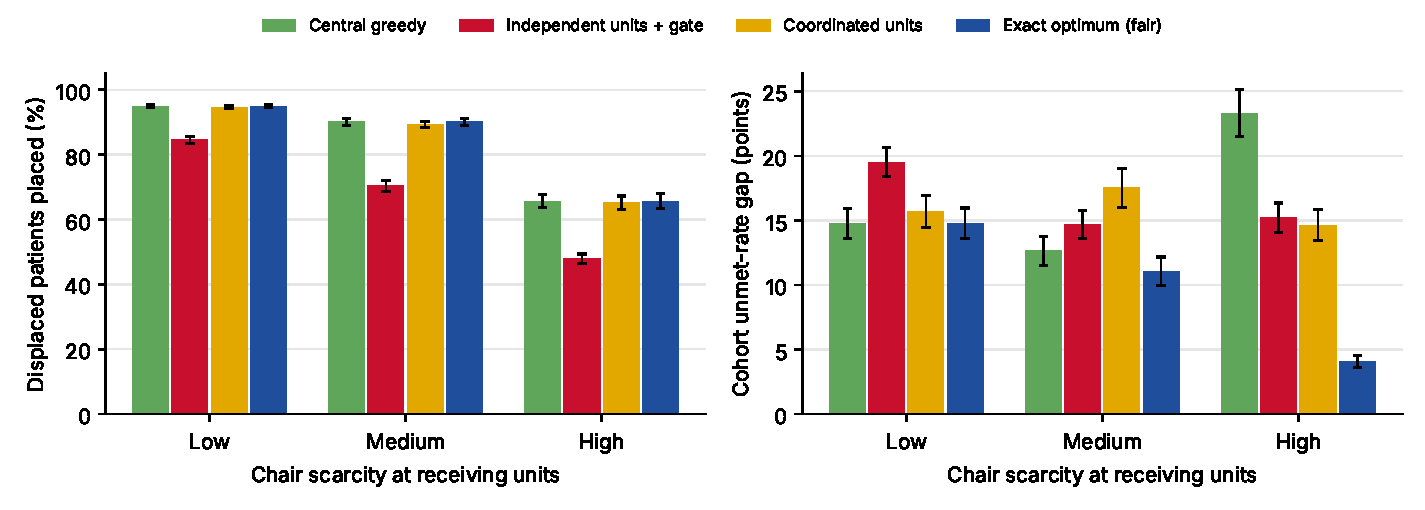
\includegraphics[width=\linewidth]{figures/fig_fulfilment_gap.pdf}
\caption{Share of displaced patients placed (left) and the cohort gap (right) by chair scarcity, with 95\%
bootstrap intervals. Each bar is 400 scenarios. ``Central greedy'' is the most-constrained greedy planner.}
\label{fig:main}
\end{figure}

\paragraph{Separate decisions lose patients.} Units acting independently placed 70.4\% of displaced
patients, 13.2 points below the optimum (95\% CI $-13.9$ to $-12.4$; Table~\ref{tab:main}). The loss has two
sources. Offers to patients who accepted elsewhere lapse, so chairs stay empty; and units book transport
against the whole fleet, so 47.8\% of plans overbooked it, by 0.94 seats on average. The gap widened with
scarcity: 4.9 points at low scarcity and 17.3 at high (Figure~\ref{fig:main}). Their cohort gap of 11.8 points
looks small only because both groups were badly served (unmet rates 30.6\% and 29.1\%).

\paragraph{A safety gate makes plans feasible, not better.} Checking the proposals against the shared fleet
before commit removed every violation but placed 67.6\%, 2.8 points fewer than without the gate, and raised
the transport group's unmet rate from 30.6\% to 38.7\%. The gate removes bookings that do not fit; it does not
look for other places.

\paragraph{Coordination recovers the loss.} Rounds of offers against a shared ledger placed 83.0\%, within 0.5
points of the optimum (paired CI $-0.6$ to $-0.4$), with every plan feasible, at 1.1 more minutes of burden per
placed patient than the fairness-first optimum.

\paragraph{Greedy planners place enough patients but not fairly.} Both greedy planners placed as many patients
as the optimum or within 0.3 points of it, but at a cost in fairness and burden. Their cohort gaps were 15.5
and 16.9 points against 10.0 for the fairness-first optimum, and they gave 5.5--5.8 more minutes of burden
per patient. Placing the most constrained patients first moved unmet patients from the transport group to the
independent group: under high scarcity it left 41.4\% of independent patients unplaced against 21.6\% of
transport patients, a gap of 23.3 points. The fairness-first optimum held the gap to 4.1 points at the same
number placed.

\paragraph{Fairness cost nothing here.} The fairness-first optimum placed the same share as the throughput
optimum in every cell and had the same mean burden to one decimal place. Under low scarcity both optima still
left a gap of about 15 points: transport seats, not chairs, were the binding constraint, and no allocation of
chairs can close that gap.

\section{Discussion}
The results separate two failure modes that are easy to conflate. When units decide separately, the main loss
is patients placed, caused by lapsed offers and collisions on a shared resource. A commit-time gate prevents
infeasible plans but does not restore placements; coordination through a shared ledger does. When a central
planner decides greedily, the number placed is close to optimal, but who goes unplaced depends on the order
rule, and an apparently sensible rule (most constrained first) can shift the burden onto a different group.
An explicit fairness objective fixed this at no cost in these scenarios, in line with the observation that
the price of fairness is often small \citep{bertsimas2011price}.

For services, the practical points are to keep a shared ledger of scarce cross-unit resources such as
transport, to plan centrally or in coordinated rounds rather than in one round of separate offers, and to
state explicitly whose unmet need is being minimised. Where transport is the binding constraint, adding seats
matters more than any allocation rule.

\section{Limitations}
The networks are synthetic: chair counts, occupancy, travel limits, the transport share and fleet size are
illustrative and not taken from any service. Travel is straight-line distance converted to minutes, with no
road network or multi-day planning. The two groups are an operational construct, and the cohort gap is not a
validated social or clinical fairness measure. Clinical priority, infection control, staffing rules and
patient preference are not modelled. Unit agents are rule-based; language-model agents are not evaluated in
this study.

\section*{Data and code availability}
Code, scenario generator, per-scenario results and figures are at
\url{https://github.com/MHKhan50/dialysisflow-agentbench} (version 0.2.0). No patient data are used.

\bibliographystyle{unsrtnat}
\bibliography{references}

\end{document}
